\begin{comment}
Multicore architectures 
cache system
sharing and false sharing
existing tools for false sharing
limitations
contributions
structures
\end{comment}

Multicore processors are ubiquitous in the whole computing spectrum, from mobile phones, personal desktops, to high-end servers. Multithreading is the de-facto programming model to exploit the massive parallelism in modern architectures.
%Multithreading is widely used to employ these ubiquitous multicore processors for high parallelism. 
However, multithreaded programs may suffer from various performance issues because of complex memory hierarchies~\cite{ibs-sc,ibs-sc2,Dramon}. Among them, false sharing is a common flaw that can significantly hurt the performance and scalability of multithreaded programs~\cite{falseshare:effect}. False sharing occurs when different threads, which are running on different cores with private caches, concurrently access logically independent words of the same cache line. When a thread modifies the data of a cache line, the cache coherence protocol (managed by hardware) silently invalidates the duplicates of this cache line in the private caches of other cores~\cite{MESI}. Thus, even if other threads access independent words of this cache line, they have to unnecessarily reload the entire cache line from the shared cache or main memory. 

Unnecessary cache coherence caused by false sharing can dramatically degrade the performance of multithreaded programs by up to an order of magnitude~\cite{falseshare:effect}. A concrete example shown in Figure~\ref{fig:penalty} also shows this catastrophic performance effect. We meant to use threads to accelerate the computation for the {\tt array}. However, when eight threads (on an 8-core machine) simultaneously access adjacent elements of {\tt array}, this program actually runs around $13\times$ slower (back bars) than its expectation (grey bars) with no false sharing.
%The performance degradation caused by false sharing can be even more severe in modern architectures that integrate multiple sockets in chip; threads in different sockets involved in false sharing cause the cache coherence occurring in main memory not shared cache.
The hardware trend, including adding more cores into the same machine, introducing the Non-Uniform-Memory-Access (NUMA) architecture, or increasing the size of a cache line, will further degrade the performance of programs with false sharing.
%, making the task of detection even more urgent. 

\begin{figure*}[htbp]
\centering
\subfigure[A Program with False Sharing]{%
   \label{fig:penaltycode}
   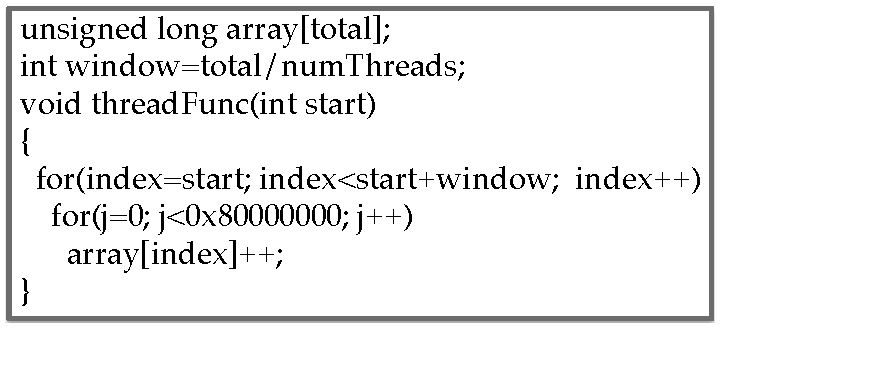
\includegraphics[width=3.1in]{figure/fscode}

}%
\hspace{20pt}
\subfigure[Performance Degradation]{%
   \label{fig:penaltyfig}
   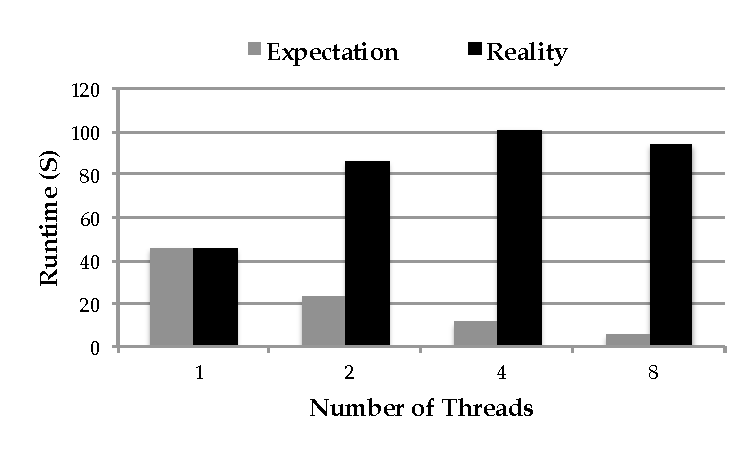
\includegraphics[width=3.1in]{figure/penalty}
}
\caption{
A false sharing example inside a multithreaded program (a) causes $13\times$ performance degradation (b) on a 8-core machine.
\label{fig:penalty}}
\end{figure*}

%\todo{Confirm the picture is readable in grey-style printing}

% Now we will talk about existing tools. 
Unlike true sharing, false sharing is generally avoidable. When threads unnecessarily share the same cache line, we can pad the data or make a thread to update its thread-private variable so that different threads can be forced to access a different cache line. Although the solution of fixing false sharing is somehow straightforward, detecting them is difficult and even impossible with manual checking, especially for a program with thousands or millions lines of code. Thus, it is very important to employ tools to pinpoint false sharing and provide insightful optimization guidance.

However, existing general-purpose tools do not provide enough details about false sharing~\cite{gprof, ibs-sc, Intel:VTune}. Existing false sharing detection tools fall short in several ways. First, most tools cannot distinguish true and false sharing, requiring substantial manual effort to identify optimization opportunities~\cite{falseshare:binaryinstrumentation1,detect:ptu,detect:intel,falseshare:binaryinstrumentation2,DProf, qinzhao, OSdetection, mldetect, Wicaksono11detectingfalse, openmp}. Second, software-only tools~\cite{falseshare:binaryinstrumentation1,falseshare:binaryinstrumentation2,falseshare:simulator, Predator} introduce very high runtime overhead, preventing them from being used in deployment environment. Third, OS-related tools have limitations, either with customized OS support~\cite{OSdetection}, or only working on special applications~\cite{Sheriff}. Fourth, no prior tool assesses the benefit from eliminating the false sharing. Without this information, many optimization efforts may yield trivial or no performance improvement.

In this paper, we present \cheetah{} to address these issues, with the following contributions:
\begin{itemize} 

% The first one is overrated. We can't do that. 
\item {\bf First Approach to Predict False Sharing Impact.} This paper introduces the first approach to predict the performance impact of fixing false sharing instances inside multithreaded programs. Based on our evaluation, \cheetah{} can precisely assess the performance improvement, with less than 10\% difference. By ruling out trivial instances, we can avoid unnecessary manual effort leading to little or no performance improvement. 

\item {\bf An Efficient and Effective False Sharing Detection Tool.} \cheetah{} is an efficient false sharing detector with only $\sim$7\% runtime overhead. \Cheetah{} utilizes the Performance Monitoring Units (PMU) that are available on modern CPU architectures to sample memory accesses. \cheetah{} can precisely and correctly report false sharing problems, by pointing out the lines of code or the name of variables with problems. 
\cheetah{} is language and compiler independent. It works on native binaries that are compiled with any optimization option. 
%which does not need custom OS,  or recompilation and changing of programs. 
\end{itemize}

\begin{figure}[htbp]
\centering
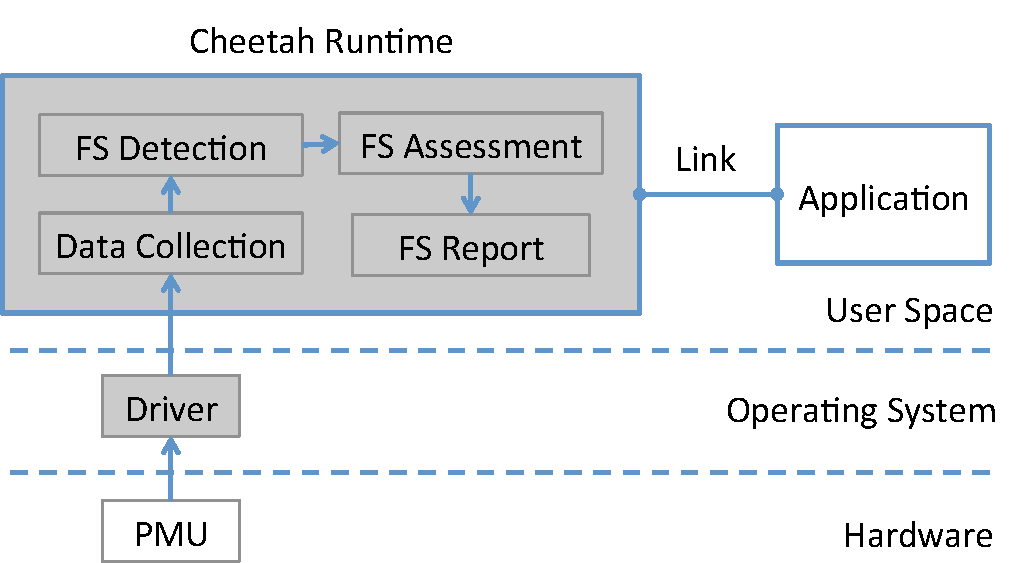
\includegraphics[width=.8\columnwidth]{figure/cheetahcomponents}
\caption{Overview of \cheetah{}'s components (shadow blocks).}
\label{fig:components}
\end{figure}


%\cheetah{} is very convenient to use. There is no need to change or recompile programs, or to modify the underlying operating system. We evaluate \cheetah{} on two well-known benchmark suites, PARSEC~\cite{phoenix-hpca} and PHOENIX~\cite{parsec}. \cheetah{} successfully identifies significant false sharing problems, while skipping problems with only trivial or no performance improvement.

%
%is very convenient to use, which is a library that can be preloaded (using \texttt{LD\_PRELOAD} or can be linked to: there is no need to change or recompile the programs, or to modify the underlying operating system.
\paragraph{\cheetah{} Overview}
Figure~\ref{fig:components} shows the overview of \Cheetah{}. \Cheetah{} is has a co-design with hardware, operating system, and the user space programs. It monitors the memory accesses via the hardware performance monitoring unit (PMU) supported address sampling. By analyzing the address samples, \cheetah{} identifies significant false sharing problems (in FS-Detection component) and quantifies their impacts to the whole program execution (in FS-assessment component).
%'s components. When the Performance Monitoring Unit (PMU) invokes an interrupt according to the pre-set sampling frequency, the ``driver'' passes all information about a memory access to the ``data collection'' module residing in \Cheetah{}'s runtime system. Upon receiving this, the ``data collection'' module filters out memory accesses relating to heap or globals, and feeds them into the ``FS detection'' module. At the end of an application or when \cheetah{} is notified to report, ``FS detection'' will examine the number of cache invalidations of each cache line, differentiate false sharing from true sharing, and pass false sharing instances to the ``FS assessment'' module. Thus, ``FS report'' module only reports false sharing instances with significant performance impact, with its predicted performance improvement after fixes for every instance. 

The remainder of this paper is organized as follows. 
%Section~\ref{sec:overview} introduces the background of false sharing and the motivation of a new detection tool. 
Section~\ref{sec:detect} describes the design and implementation of false sharing detection tool. Section~\ref{sec:predictimprove} introduces how \cheetah{} assesses the performance impact of a false sharing instance. Section~\ref{sec:eval} presents experimental results, including effectiveness, performance overhead, and the precision of assessment. Section~\ref{sec:discuss} addresses main concerns on hardware dependence, performance and effectiveness. Section~\ref{sec:relatedwork} discusses related work and Section~\ref{sec:conclusion} concludes this paper. 



